\documentclass[12pt]{article}
\usepackage[paper=letterpaper,margin=1.5cm]{geometry}
\usepackage{amsmath}
\usepackage{amssymb}
\usepackage{amsfonts}
\usepackage{mathtools}
\usepackage[utf8]{inputenc}
\usepackage{newtxtext, newtxmath}
%\usepackage{enumitem}
\usepackage[shortlabels]{enumitem}
\usepackage{titling}
\usepackage{graphicx}
\usepackage[colorlinks=true]{hyperref}
\usepackage{setspace}
\usepackage{braket}
\usepackage{color}
\usepackage{listings}
\usepackage{mathrsfs}
\usepackage{stackengine}
\usepackage{afterpage}

\setstackEOL{\\}

\definecolor{dkgreen}{rgb}{0,0.6,0}
\definecolor{gray}{rgb}{0.5,0.5,0.5}
\definecolor{mauve}{rgb}{0.58,0,0.82}

\lstset{frame=tb,
  language=Python,
  aboveskip=3mm,
  belowskip=3mm,
  showstringspaces=false,
  columns=flexible,
  basicstyle={\small\ttfamily},
  numbers=none,
  numberstyle=\tiny\color{gray},
  keywordstyle=\color{blue},
  commentstyle=\color{dkgreen},
  stringstyle=\color{mauve},
  breaklines=true,
  breakatwhitespace=true,
  tabsize=3
}
\setlength{\droptitle}{-6em}

\newcommand{\hop}{\vspace{1mm}}
\newcommand{\jump}{\vspace{5mm}}
\newcommand{\R}{\mathbb{R}}
\newcommand{\C}{\mathbb{C}}
\newcommand{\bt}{\textbf}
\newcommand{\lm}{\lambda}
\newcommand{\ep}{\varepsilon}
\definecolor{cit}{rgb}{0.05,0.2,0.45}
\addtolength{\jot}{1em}
\newcommand{\solution}[1]{

\vspace{5mm}
\medskip\noindent{\color{cit}\textbf{Solution:} #1}}

\newcounter{tmpctr}
\newcommand\fancyRoman[1]{%
  \setcounter{tmpctr}{#1}%
  \setbox0=\hbox{\kern.1pt\textsf{\Roman{tmpctr}}}%
  \setstackgap{S}{-.2pt}%
  \Shortstack{\rule{\dimexpr\wd0+.1ex}{.5pt}\\\copy0\\
              \rule{\dimexpr\wd0+.1ex}{.5pt}}%
}

\newcommand{\Id}{\fancyRoman{2}}

% Enter the specific assignment number and topic of that assignment below, and replace "Your Name" with your actual name.
\title{STAT 31410: Homework 1}
\author{Caleb Derrickson}
\date{October 8, 2023}

\begin{document}
\onehalfspacing
\maketitle

{\color{cit}\vspace{2mm}\noindent\textbf{Collaborators:}} The TA's of the class, as well as Kevin Hefner, Nathan Suhr, and Steven Lee.

\jump
For this problem set, we consider the equation for an idealized pendulum
\begin{align}
    \frac{d^2\theta}{dt^2} = -\frac{g}{\ell(t)}sin(\theta), \label{Original ode}
\end{align}

where the length of the moment arm, $l$, varies periodically according to

\begin{align}
    \ell (t) = \ell_0(1 + \ep \cos(\omega t)), \hspace{5mm} \ep \ll 1.    \label{length approx}
\end{align}

This might be a good model of a child on a swing, trying to pump energy into it by repeatedly
standing up and then squatting back down with some appropriate rhythm, to be determined.

\jump
\centerline{\noindent}%
\makebox[\textwidth]{
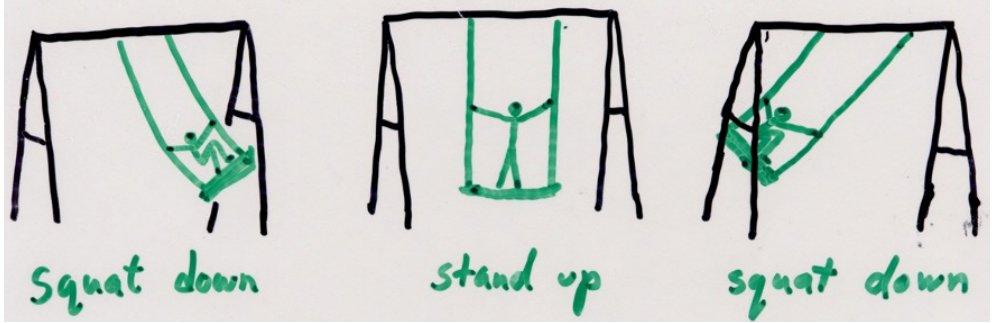
\includegraphics[scale = 0.6]{Images/swing.PNG}
}
\jump

\begin{enumerate}[]
    \item Make an approximation where you keep only the leading order term in $\ep$, i.e linearize about $\varepsilon$ = 0. Then choose a non-dimensionalization of time that puts (1) into this form:

    \begin{align}
        \ddot{\theta} = -(\alpha + \beta \cos(\tau))\sin(\theta),   \label{linearish}
    \end{align}

        where you define the dimensionless parameters $\alpha$ and $\beta$ in terms of the original parameters $g$, $\ell_0$, $\varepsilon$ and $\omega$. Re-write the second order equation \ref{linearish} as two first order equations for the angle $\theta$ and the angular speed $\Omega \equiv \dot{\theta}$. For $\beta$ = 0, derive a conserved quantity, the energy of the pendulum, denoted $E(\theta, \Omega)$. Write an equation for $\dot{E}$ that applies if $\beta \neq 0$.
        \begin{solution}

        Since we are taking $\ep \ll 1$ from \ref{Original ode}, we can define a function $f(\ep)$ on which we will expand using ordinary Taylor expansion. Here, I will define $f(\ep)$ as:
        \begin{align}
            f(\ep) = \frac{1}{1 + \ep \cos(\omega t)},
        \end{align}

        where it is understood that $\cos(\omega t)$ is a constant in this sense. Note that we are \textit{linearizing} with respect to $\theta$, so we can drop all terms of higher order. Thus, 

        \begin{align}
            f(\ep) &= \sum_{n = 0}^\infty \ep^n\frac{d^nf}{d\ep^n} \Big\rvert_{\ep = 0} \nonumber \\
            &= f(\ep = 0) + \ep\frac{df}{d\ep} \Big\rvert_{\ep = 0} + O(n^2)  \nonumber \\
            &= 1 - \ep \bigg[ \frac{\cos(\omega t)}{(1 + \ep\cos(\omega t))^2} \bigg]_{\ep = 0}  \nonumber \\
            & = 1 - \ep \cos(\omega t) \label{Expansion} 
        \end{align}

        We can then plug \ref{Expansion} into \ref{Original ode} to obtain,

        \begin{align}
            \ddot{\theta} = -\frac{g}{\ell_0}\Big(1 - \ep \cos(\omega t)\Big)\sin(\theta). \label{before parameters}
        \end{align}

        From \ref{before parameters}, we can define three dimensionless parameters: $\tau, \alpha, \beta$. $\tau$ will take the place of the argument inside the cosine term of \ref{before parameters}, while $\alpha$ and $\beta$ will clean up any extraneous terms. We will first redefine the ratio of $g$ and $\ell_0$ as the resonance frequency of our state, $\omega_0$.
        
        \begin{align*}
            \omega_0^2 = \frac{\ell_0}{g}.    
        \end{align*}

        Then we will take $\tau$ as $\tau = \omega t$. Note that we are taking time derivatives, so this re-parameterization affects what we are differentiating by. 

        \begin{align*}
            \tau = \omega t \implies d\tau = \omega dt \iff \frac{1}{\omega}\frac{d}{d\tau} = \frac{d}{dt}.
        \end{align*}

        Applying these to \ref{before parameters}, we get,

        \begin{align}
            \ddot{\theta} = -\Big(\frac{\omega_0}{\omega} \Big)^2 \big( 1 - \ep \cos(\tau) \big) \sin(\theta).  \label{before alphabeta}
        \end{align}

        We can then define $\alpha, \beta$ as,

        \begin{align}
            \alpha = \bigg(\frac{\omega_0}{\omega}\bigg)^2, \hspace{10mm} \beta = \alpha\ep
        \end{align}

        Note that, as suggested by the TA's, to take $\beta$ as a positive constant. The negative can be recovered by shifting $\tau$ by $\pi$, meaning $\tau = \omega t + \pi$. This shift will change nothing else in our analysis, hopefully. Also, when taking time derivates for the rest of this homework, I am specifically referring to taking the $\tau$ derivative. Thus, our second order differential equation is, 

        \begin{align}
            \ddot{\theta} = -\big(\alpha + \beta \cos(\tau)\big)\sin(\theta),   \label{second order ode with new parameters}
        \end{align}

        matching \ref{linearish}. 

        Our next goal is to re-write \ref{second order ode with new parameters} as two first order equations for $\theta$ and the angular speed $\Omega \equiv \dot{\theta}$. This can be achieved quite easily - our system is now. 
        \begin{equation}
        \begin{cases}
            \dot{\theta} = \Omega, \\
            \dot{\Omega} = -\big(\alpha + \beta \cos(\tau)\big)\sin(\theta) \label{Nonlinear system}
        \end{cases}    
        \end{equation}

        Our next goal is to find a conserved quantity for $\beta = 0$. This quantity will be the energy of our system (or rather, an approximation of it) and will be denoted as $E$. From the lectures, our energy is the sum of kinetic and potential energies, in just the $\theta$ dimension. Potential can be found by integrating the (negative) right-hand-side of \ref{second order ode with new parameters} by our spacial parameter. 

        \begin{align}
            \implies V(\theta) &= \int \alpha\sin(\theta) \ d\theta \nonumber\\
            &= -\big(\alpha + \beta\cos(\tau))\cos(\theta)
        \end{align}

        The energy is now,

        \begin{align}
            E(\theta, \Omega) &= \frac{1}{2} \dot{\theta}^2 + V(\theta),    \nonumber   \\
            E(\theta, \Omega) &= \frac{1}{2} \Omega^2 -\alpha\cos(\theta).
        \end{align}

        Where the instantaneous change in energy (with respect to time) is,

        \begin{align}
            \dot{E}(\theta, \Omega) &=  \frac{d}{d\tau}\bigg[ \frac{1}{2}\Omega^2 - \alpha\cos(\theta) \bigg]  \nonumber\\
            &= \Omega\dot{\Omega} - \alpha\frac{d}{d\tau}\bigg[ \cos(\theta) \bigg] \nonumber\\
            &= -\Omega\big(\alpha + \beta \cos(\tau)\big)\sin(\theta) + \alpha\sin(\theta)\dot{\theta}\nonumber\\
            &= -\beta\Omega\cos(\tau)\sin(\theta) \label{Edot}
        \end{align}
        \end{solution}

        \hrule
        
        \jump
        For the child in the swing picture, is the energy $E$ (instantaneously) increasing or decreasing or neither in each of the frames shown? Try making a rough sketch of the time course of each of these quantities: $\theta(t), \Omega(t), \ell(t)$ and $E(t)$, assuming a periodic motion of the swing as well as the swinger. What is the period of the swing motion compared to the period of $\ell(t)$? Are they the same?

        \begin{solution}
            As a means of faithfully showing the plots, I used matplotlib to create them. Note I am not showing the numerical values of the functions, since they are not enlightening. Note the function $\ell(t)$ is bounded by $1 \pm \ep$. My code is shown below, followed by the generated plots.

            \jump

            Note that these are here purely as a heuristic. As we expect the length of the pendulum arm to be the greatest while the child is squatting down, and minimal when the child to be standing up. Squatting down should correlate to maximum values of theta, and standing up should correlate to minimum values of theta. We can see this represented in the plots of length and theta. Since $\dot{\theta} = \Omega$, we should see maxed values of $\omega$ when $\theta$ = 0, which is shown. Energy is slightly different. When $E$ = 0, the kinetic energy is equal to its potential, which happens going to and coming from max values of $\theta$. It's maximal values should then be when either the kinetic or potential energies are maximized, lining up with values $\theta = -\pi/2, \ 0, \ \pi/2$. Regardless, in an entire swing interval, when going from $-\pi/2$ to $\pi/2$, we should hit the zeros of $E$ four times, indicating that the energy runs with frequency four times that of $\theta$, twice the frequency of $\ell$. Though this seems to not be represented in the plot of energy, I expect my rationality to be a better interpretation. 

            From our calculation of $\dot{E}$, we can inspect the change of the energy in the given frames of the system. Note that we are to expect the system to achieve its maximum heights in the first and third frames. In the first frame, we can argue the change in energy is zero, as shown by \ref{Edot}, $\Omega$ should be zero. This is also seen in the third frame. The second frame shows the child at $\theta = 0$, thus $\sin(\theta) = 0$, making our $\dot{E}$ also zero. 
        \end{solution}
        \jump
        \begin{lstlisting}

        import matplotlib.pyplot as plt
        import numpy as np
        import pandas as pd
        %matplotlib inline

        def ell(tau, ep):
            return (1 + ep * np.cos(2 * tau))
        def Omega(tau, ep):
            return -1*(np.sin(tau))
        def energy(tau, ep):
            return 0.5 * Omega(tau, ep) **2 - np.cos(theta(tau))
        def theta(tau):
            return np.cos(tau)

        ep = 0.1
        tau = np.linspace(-np.pi * 2, np.pi * 2, 200)
        tau_ticks = np.arange(-np.pi * 2, np.pi * 2, np.pi/2)
        tau_ticks_label = [f'0' if n == 0 else f'-pi/2' if n == -1 else f'pi/2' if n == 1 else f'{int(n/2)}pi' if n%2 == 0 else f'{int(n)}pi/2' for n in tau_ticks / (np.pi / 2)] 
        
        plt.figure(figsize=(10, 8))
        plt.subplots_adjust(hspace=0.5)
        
        plt.subplot(2, 2, 1)
        plt.plot(tau, ell(tau, ep), 'b-', label = "Length")
        plt.plot(tau, [np.mean(ell(tau, ep)) for _ in range(len(tau))], 'k--')
        plt.xlabel("tau")
        plt.title("Length")
        plt.yticks([])  
        plt.xticks(tau_ticks, tau_ticks_label)
        
        plt.subplot(2, 2, 2)
        plt.plot(tau, Omega(tau, ep), 'r-', label = "Omega")
        plt.plot(tau, 0 * tau, 'k--')
        plt.xlabel("tau")
        plt.title("Omega")
        plt.yticks([])  
        plt.xticks(tau_ticks, tau_ticks_label)
        
        plt.subplot(2, 2, 3)
        plt.plot(tau, energy(tau, ep), 'g-', label = "Energy")
        plt.plot(tau, [np.mean(energy(tau, ep)) for _ in range(len(tau))], 'k--')
        plt.xlabel("tau")
        plt.title("Energy")
        plt.yticks([])  
        plt.xticks(tau_ticks, tau_ticks_label)
        
        plt.subplot(2, 2, 4)
        plt.plot(tau, theta(tau),  'm-', label = "Theta")
        plt.plot(tau, 0 * tau, 'k--')
        plt.xlabel("tau")
        plt.title("Theta")
        plt.yticks([])  
        plt.xticks(tau_ticks, tau_ticks_label)
        
        plt.show()

        \end{lstlisting}
        
        \jump
        \centerline{\noindent}%
        \makebox[\textwidth]{
        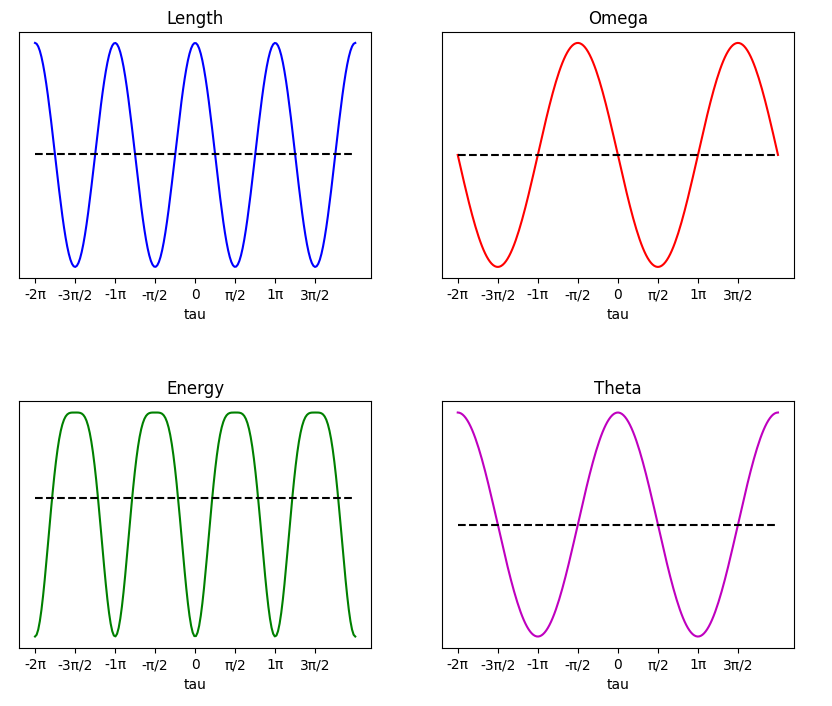
\includegraphics[scale = 0.6]{Images/homework1 heuristic plots.PNG}
        }
        \jump

        \item Linearize your system of first order equations about the equilibrium position $\theta = \Omega = 0$ to obtain a linear non-autonomous system to study:

        \begin{align}
            \frac{d\textbf{x}}{d\tau} = A(\tau)\textbf{x}, \label{Linearized system}
        \end{align}

        where $A(\tau) = A(\tau + T)$ is a 2$\times$2 T-periodic matrix, and $\textbf{x} \in \R^{2}$ is your state space vector. What is T for your non-dimensional problem?
        
        \jump

        \begin{solution}
        
            In preparation for this, we wrote out our ``pseudo system" as \ref{Nonlinear system}. From this, we are only interested in small perturbations of $\theta$ and $\Omega$ around $\theta = \Omega = 0$. Thus, we can replace functions dependent on $\theta$ and $\Omega$ with their Taylor Expanded equivalent, up to linear term. From \ref{Nonlinear system}, the only function is $\sin(\theta)$, which can be approximated by $\sin(\theta) \approx \theta$ under our assumptions. Therefore we have,

            \begin{align}
                \begin{pmatrix}
                    \dot{\theta}    \\
                    \dot{\Omega}
                \end{pmatrix}
                \hspace{3mm}
                =
                \hspace{3mm}
                \begin{pmatrix}
                    0   &1  \\
                    -\big( \alpha + \beta\cos(\tau)\big) &0
                \end{pmatrix}
                \begin{pmatrix}
                    \theta  \\
                    \Omega
                \end{pmatrix}   \label{Linear system}
            \end{align}

            It is quite easy to see that our state vector, \textbf{x} is just $(\theta, \Omega)^t \in \R^2$, where $t$ denotes the transpose. It is also noted that our system $A(\tau)$ is periodic, with period $T = 2\pi$.
        \end{solution}

        \jump
        \hrule
        
        \jump
        Briefly summarize what Floquet theory tells us about the form of the solutions of \ref{Linear system}.

        \begin{solution}
        
            Floquet theory tells us that there exists some periodicity in our solutions. Since our system is periodic (with period $T = 2\pi$), the general form of the solutions is given by theorem 2.36 in the course book.

            \begin{align}
                \upPhi (t,0) = \mathscr{P}(t)e^{tB}, 
            \end{align}

            where $\mathscr{P}$ is a $T$-periodic matrix and $B = \frac{1}{T} \ln M$, where M is the monodromy matrix: $M \equiv \upPhi(T,0)$. 
        \end{solution}

        \item Let $\upPhi(\tau)$ be the fundamental matrix solution associated with the linear problem \ref{Linear system} that satisfies $\upPhi(0) = \Id$, the 2×2 identity matrix. Derive and then solve a first order ordinary differential equation for $det(\upPhi)$.

        \jump

        \begin{solution}
          
        This is done in the book as the proof of Abel's formula, so I will transcribe the proof in my own words. 

        \jump
        First we re-write det($\upPhi$) into an equivalent form, 
        
        \begin{align}
            \text{det($\upPhi$) = } \sum_{j = 1}^nc_{ij}\varphi_{ij}, \label{detupphi}
        \end{align}

        where $c_{ij}$ is the co-factor of the $i,j$-th entry of $\upPhi$. Note that \ref{detupphi} can be taken over any row of $\upPhi$, thus if we decouple the respective indices row entries of $\varphi_{ij}$ and $c_{ij}$, we get,

        \begin{align}
             \text{det($\upPhi$) $\delta_{ik}$= } \sum_{j = 1}^nc_{ij}\varphi_{kj}, \label{deltadetupphi}
        \end{align}

        where $\delta_{ik}$ is the Kronnecker delta of $i$ and $k$. Furthermore, since the only term in \ref{detupphi} which depends on $\varphi_{ij}$ is exactly the term $c_{ij}\varphi_{ij}$, we can write,

        \begin{align}
            \frac{\partial}{\partial\varphi_{ij}}\text{det($\upPhi$) = }c_{ij}. \label{partialdetphi}
        \end{align}

        Therefore, using the chain rule and \ref{partialdetphi}, we can write the time derivative of det($\upPhi$) as,

        \begin{align*}
            \frac{d}{dt}\text{det($\upPhi(t)$)} = \sum_{i = 1}^n\sum_{j = 1}^n c_{ij}(t)\frac{d}{dt}\varphi_{ij}.
        \end{align*}

        Note that the fundamental matrix has columns of the linearly independent solutions of \ref{Linear system}, thus 
        \[
        \frac{d}{dt}\varphi_{ij}(t) = A(t)\upPhi(t) = \sum_{k = 1}^n a_{ik}\varphi_{kj}(t)
        \]

        This can then be substituted into our ODE, making it,

        \[
        \frac{d}{dt}\text{det($\upPhi(t)$)} = \sum_{i, j, k}^n c_{ij}(t)a_{ik}(t)\varphi_{kj}(t),
        \]

        where I have compressed the triple sum for legibility. Rearranging these terms and noting that $a_ik$ does not depend on the $j$ summation implies,

        \[
        \frac{d}{dt}\text{det($\upPhi(t)$)} = \sum_{i,k = 1}^na_{ik}(t)\sum_{j = 1}^n c_{ij}(t)\varphi_{kj}(t).
        \]

        The inner summation is equivalent to \ref{deltadetupphi}, thus,

        \[        
        \frac{d}{dt}\text{det($\upPhi(t)$)} = \sum_{i,k = 1}^na_{ik}(t)\delta_{ik}\text{det($\upPhi$)}.
        \]

        det($\upPhi$) can be taken out of the summation, and the Kronnecker delta collapses the summation to the case where $i = k$, so,

        \[        
        \frac{d}{dt}\text{det($\upPhi(t)$)} = \text{det($\upPhi$)}\sum_{i = 1}^na_{ii}(t).
        \]

        This summation is exactly the trace of A, then our ODE is exactly

        \[
        \frac{d}{dt}\text{det($\upPhi(t)$)} = \text{det($\upPhi$)}\text{tr($A$)}.
        \]

        Treating this as a separable ODE, and nothing the trace of a matrix is a scalar, we get,

        \begin{align}
        &\frac{d(\text{det($\upPhi$)})}{\text{det($\upPhi$)}} = \text{tr($A(t)$)}dt, \nonumber\\
         \iff \int &\frac{d(\text{det($\upPhi$)})}{\text{det($\upPhi$)}} = \int_{t_0}^t \text{tr($A(s)$)}ds, \nonumber\\
         \iff \hspace{5mm}&\text{det($\upPhi$)} = \text{exp}\bigg[ \int_{t_0}^t\text{tr($A(s)$)$ds$}\bigg] \label{Abelresult}
        \end{align}

        This is the result of Abel's theorem, completing the proof. 
        \end{solution}

        \jump
        \hrule
        \jump
        What can you say, based on this, about the eigenvalues $\mu$ of the monodromy matrix $M \equiv \upPhi(T,0)$?

        \jump
        \begin{solution}
        
            By our Linear system, $A(s) = 0$, so the determinant of our fundamental matrix, by \ref{Abelresult}, is equal to $e^0 = 1$ for any time $t$. Thus, for $t = 0$, the monodromy matrix has determinant 1. This then breaks down into two cases, depending if the eigenvalues are real or complex.

            In the real case, this means that $\mu_1$ and $\mu_2$ are inverses of each other, i.e. $\mu_1 = \frac{1}{\mu_2}$. As explained briefly in the lectures, this solution will lead to instability in our solutions. 

            In the complex case, this means $\mu_1 = \overline{\mu_2}$, i.e. they are complex conjugates of each other. This will mean our solutions are stable, leading to some oscillation.
        \end{solution}

        \jump
        \hrule
        \jump
        If we add some linear damping to the problem so that \ref{linearish} becomes

        \begin{align}
            \ddot{\theta} = -\bigg(    \alpha + \beta\cos(\tau)\bigg)\sin(\theta) - \gamma\dot{\theta}     \hspace{5mm} \gamma > 0,
        \end{align}

        What can you say about the determinant of the Monodromy matrix associated with the linearized problem in that case?

        \jump
        \begin{solution}

            Under the approximation we employed to derive \ref{Linear system}, we'll take $\sin(\theta) \approx \theta$. Also, we will decompose this second order ODE into two first order by the substitution $\Omega = \dot{\theta}$, $\dot{\Omega} = -(\alpha + \beta\cos(\tau))\theta - \gamma \Omega$. Thus our system is now.

            \begin{align}
                \begin{pmatrix}
                    \dot{\theta} \\
                    \dot{\Omega}
                \end{pmatrix}
                \hspace{3mm}
                = 
                \hspace{3mm}
                \begin{pmatrix}
                    0    &1 \\
                    -(\alpha + \beta\cos(\tau)) &-\gamma
                \end{pmatrix}
                \begin{pmatrix}
                    \theta  \\
                    \Omega
                \end{pmatrix}
                \label{damplinearsystem}
            \end{align}

            Thus, by \ref{Abelresult}, 
            \begin{align}
                \text{det(M)} &= \text{det($\upPhi(T,0)$) = } \exp\Bigg[-\int_0^T \gamma \text{ds}\Bigg] \nonumber\\
                &=e^{-\gamma T}
            \end{align}
        \end{solution}

        \jump
        \hrule
        \jump

     Very briefly discuss what type of stability claims, about the equilibrium $\theta = \Omega = 0$, can be made from an analysis of the solutions of \ref{Linearized system} in the case of $\gamma = 0$ and the case of $\gamma > 0$. Recall that there are different types of “stability”, e.g. Lyapunov stability, asymptotic stability, linear stability, as well as instability. Later we will be looking at some results that tell us when it is enough to examine the linearized problem to determine the stability properties of an equilibrium of the nonlinear problem. We will also be interested in cases where that is not enough.

     \begin{solution}
     
         To start off my brief discussion, I will summarize these two classes of stability. Lyapunov stability claims that there exists a neighborhood centered at $x^*$ such that $x^*$ is a zero of of \ref{Linearized system} within which our solution resides for any $t$. Asymptotic stability takes the Lyapunov stability and adds the condition that a solution will tend to $x^*$ as $t \rightarrow \infty$. So or the case of $\gamma = 0$, our system will be only Lyapunov stable if the Floquet multipliers are complex. If they are real, the system will only have unstable solutions. When we take $\gamma > 0$, the real case stays the same, but the complex case will graduate to asymptotic stability. This are due to our calculation above. 
     \end{solution}

\jump
\hrule
\jump
\item The remainder of this problem involves numerical computations for the linearized problem \ref{Linearized system}. On an appropriate grid of parameter values $(\alpha, \beta)$ numerically compute the Monodromy matrix and its eigenvalues in order to estimate the boundary separating parameter regions where solutions are bounded vs. unbounded. Can we assume $\alpha$ and/or $\beta$ is positive?

You should find “resonance tongues” in the $(\alpha, \beta)$ parameter plane that correspond to parameters where solutions of the linear problem grow exponentially. Along the way, check how
well your numerical results match the analytic ones on det(M) from part 3.

\begin{solution}

    As a quick mention. We specifically chose both $\alpha$ and $\beta$ to be positive when we made our shift in $\tau$. The code for generating the boundaries of bounded and unbounded solutions. I had the help of Steven Lee in generating these plots. The code to generate the plots are shown first.

    We can see the "resonance tongues", boundaries of the unbounded and bounded regions in \ref{png:bounded_vs_unbounded_solns}. We can also investigate the numerical accuracy of the products of the eigenvalues. This is shown in \ref{png:mag_plots}. For both unbounded and bounded solutions, we can see product of the eigenvalues to be within 1e-6 of 1. 
\end{solution}
\jump

\begin{lstlisting}
#Function to model the system
def system(Y, t, a, b):
    x, y, phi11, phi12, phi21, phi22 = Y

    dxdt = y
    dydt = -(a + b * np.cos(t)) * x
    dphi11dt = phi12
    dphi12dt = -(a + b * np.cos(t)) * phi11
    dphi21dt = phi22
    dphi22dt = -(a + b * np.cos(t)) * phi21

    return [dxdt, dydt, dphi11dt, dphi12dt, dphi21dt, dphi22dt]
    
#Calculates the monodromy matrix from given alpha and beta
def calcualte_monodromy_matrix(alpha, beta):
    #Setting the period
    T = 2 * np.pi
    time = np.linspace(0, T, 1000)
    Y0 = [0, 1, 1, 0, 0, 1]  # initial conditions: [x0, y0, phi11, phi12, phi21, phi22]

    sol = odeint(system, Y0, time, args=(alpha, beta))

    M = np.array([[sol[-1, 2], sol[-1, 3]],
                  [sol[-1, 4], sol[-1, 5]]])
    return M

#Set up the values for alpha
alpha_span = np.linspace(0, 4, 1000)
beta_span = np.linspace(0, 4, 1000)

#Arrays to categorize solutions by choice of beta, alpha
bounded_solns = []
unbounded_solns = []
unbounded_eigenvals = []
bounded_eigenvals = []

for alpha in alpha_span:
    for beta in beta_span:
        # Calculate mono matrix
        monodromy = calcualte_monodromy_matrix(alpha, beta)
        
        #Extracting eigenvalues
        eigenvalues = np.linalg.eigvals(monodromy)
        
        #saving off eigenvalues
        eigenvals.append(eigenvalues)
        
        #Checking magnitudes to see distance from 1.0
        magnitudes = np.abs(eigenvalues)
        
        if all(np.isclose(magnitudes, 1.0, atol=1e-3)):
            bounded_solns.append((alpha, beta))
            bounded_eigenvals.append(magnitudes)
        else:
            unbounded_solns.append((alpha, beta))
            unbounded_eigenvals.append(magnitudes)
            
bounded_solns = np.array(bounded_solns)
unbounded_solns = np.array(unbounded_solns)

plt.scatter(bounded_solns[:, 0], bounded_solns[:, 1], color='blue', label='Bounded')
plt.scatter(unbounded_solns[:, 0], unbounded_solns[:, 1], color='red', label='Unbounded')
plt.xlabel('alpha')
plt.ylabel('beta')
plt.legend()
plt.title('Regions of Bounded vs. Unbounded Solutions')
plt.show()
\end{lstlisting}

\jump
\begin{lstlisting}
#Code to generate the numerical distance of Det(M) from 1
unbounded_mag = [e1*e2 - 1 for e1, e2 in unbounded_eigenvals]
bounded_mag = [e1*e2 - 1 for e1, e2 in bounded_eigenvals]
fig, axs = plt.subplots(2)
fig.suptitle('Eigenvalue Product Distances from 1')
axs[0].plot(np.abs(unbounded_mag), label = "unbounded")
axs[1].plot(np.abs(bounded_mag), label = "bounded")
\end{lstlisting}

\begin{figure}[ht]
\centering
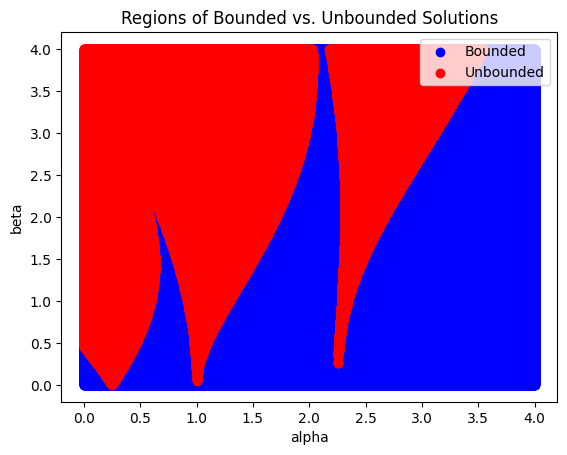
\includegraphics[scale = 0.8]{Images/bounded_vs_unbounded_solns.png}
\label{png:bounded_vs_unbounded_solns}
\caption{"Resonance Tongues"}
\end{figure}
\vspace{\floatsep}

\begin{figure}[!h]
\centering
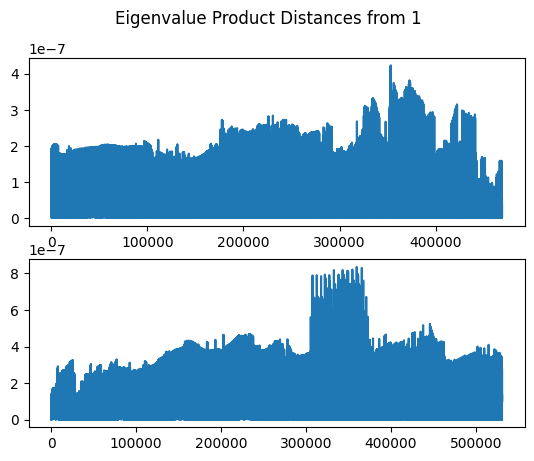
\includegraphics[scale = 0.7]{Images/unbounded_bounded_ev_plots.png}
\label{png:mag_plots}
\caption{Above is unbounded eigenvalues, below is bounded eigenvalues.}
\end{figure}

\vspace{\floatsep}
\clearpage
\jump
\hrule
\jump

For $\beta$ = 0.1, plot the real and imaginary parts of the Floquet multipliers as a function of $\alpha$; make sure to choose a large enough range of $\alpha$ values to capture the first 3 resonance tongues. (You should find that they are associated with particular values of $\alpha$; for example the first resonance tongue is associated with $\alpha$ = 0.25.) What are the Floquet multipliers on the boundary between the stable and unstable regions, for each of the tongues? What can you say about the period of the solutions on the boundaries?

\jump
\begin{solution}
    
I modified the code for generating the "Resonance tongues" plot to instead just capture the real and imaginary parts of the Floquet multipliers for $\alpha$ up to 2. Setting $\beta$ = 0.4, we see not only the first resonance tongue appear for $\alpha$ = 0.25, but also the second resonance tongue at $\alpha$ = 1.0. I could not capture the third resonance tongue, however, due to keeping a constant beta. The code to generate this is shown below, followed by the resulting plots.

Interestingly enough, the imaginary part of the Floquet multipliers collapse along the boundary of the bounded and unbounded solutions, while the real part take on an elliptic shape. It seems that, as we increase the value of $\beta$, we are getting increasingly higher ``slices" of \ref{png:bounded_vs_unbounded_solns}. I modified the targeted value of $\beta$ to capture the second tongue. This characteristic does not hold for higher values of $\alpha$, however, but we can see that the period of these elliptic shapes only increases, requiring higher values of $\beta$ to capture. 

\end{solution}

\jump
\begin{lstlisting}
#Function to model the system
def system(Y, t, a, b):
    x, y, phi11, phi12, phi21, phi22 = Y

    dxdt = y
    dydt = -(a + b * np.cos(t)) * x
    dphi11dt = phi12
    dphi12dt = -(a + b * np.cos(t)) * phi11
    dphi21dt = phi22
    dphi22dt = -(a + b * np.cos(t)) * phi21

    return [dxdt, dydt, dphi11dt, dphi12dt, dphi21dt, dphi22dt]


#Calculates the monodromy matrix from given alpha and beta
def calcualte_monodromy_matrix(alpha, beta):
    #Setting the period
    T = 2 * np.pi
    time = np.linspace(0, T, 100)
    Y0 = [0, 1, 1, 0, 0, 1]  # initial conditions: [x0, y0, phi11, phi12, phi21, phi22]

    sol = odeint(system, Y0, time, args=(alpha, beta))

    M = np.array([[sol[-1, 2], sol[-1, 3]],
                  [sol[-1, 4], sol[-1, 5]]])
    return M


#Set up the values for alpha
alpha_span = np.linspace(0, 2, 500)
beta = 0.4
real_eigenvals = []
imag_eigenvals = []

for alpha in alpha_span:
    # Calculate mono matrix
    monodromy = calcualte_monodromy_matrix(alpha, beta)

    #Extracting eigenvalues

    eigenvalues = np.linalg.eigvals(monodromy)

    #saving off eigenvalues
    for val in eigenvalues: 
        real_eigenvals.append(tuple([alpha, val.real]))
        imag_eigenvals.append(tuple([alpha, val.imag]))
        
fig, axs = plt.subplots(2, figsize=(12,8))
fig.suptitle('Floquet multipliers for beta = {}'.format(beta))
axs[0].scatter(*zip(*real_eigenvals))
axs[0].set_xlabel("alpha")
axs[0].set_ylabel("Real")

axs[1].scatter(*zip(*imag_eigenvals))
axs[1].set_xlabel("alpha")
axs[1].set_ylabel("Imaginary")

\end{lstlisting}

\jump
\begin{figure}[!ht]
\centering
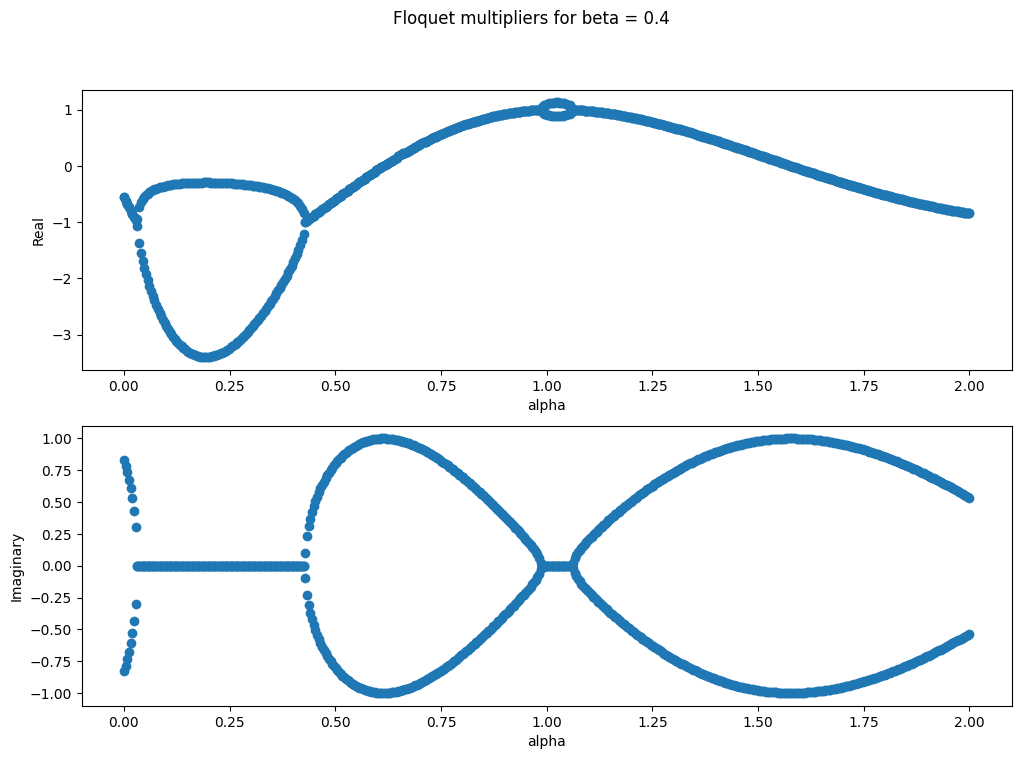
\includegraphics[scale = 0.5]{Images/real_imag_floquet_mutipliers.png}
\caption{Real and Imaginary values for Floquet multipliers. }
\label{png:real_imag_plots}

\end{figure}

\vspace{\floatsep}
\clearpage

\item The following are examples of more open-ended questions and you are encouraged to explore
at lease one of them, and/or pose and answer your own:
\begin{enumerate}[(b)]
    \item For this, let’s return to the child on the swing modeled by the nonlinear equation \ref{linearish}
rather than the linearized model \ref{Linearized system} that assumes a small angle approximation. Choose a value of $\alpha$ inside the first resonance tongue for $\beta = 0.1$. Choose an initial condition corresponding to a small angle for the pendulum. Solve this initial value problem numerically and plot $\theta(t)$ (and/or $E(t)$ and/or $\Omega(t)$ and/or $\ell(t)$) for some time interval and compare with the numerical solution of the linearized problem. It could be especially interesting to think about resonant forcing in the context of Problem Set $\#$0 where you computed the period of the pendulum as a function of its amplitude, for instance.

\jump
\begin{solution}

    For this problem, I started from scratch and numerically solved both the linear and nonlinear systems for $\alpha = 0.25, \ \beta = 0.2$. I chose these numbers just to give slightly different results, which as shown in \ref{png:bounded_vs_unbounded_solns}, should behave similarly to the requested values. I chose initial conditions $\theta_0 = \pi/10$ and $\Omega_0 = 1$. The code which solves the two systems is shown below, followed by the generated plots. Unfortunately, there is something flawed in my code, which resulted from switching to interactive plotting for various values of the initial conditions. In this transition I had to update some packages, so this might be the cause of the issue. Fortunately enough, I saved off the plots before this problem happened, so I have something legible to present. The ``better" plots are shown in \ref{png:nonlinear_vs_linear_systems}, while the plots which contain the error are shown in \ref{png:nonlinear_vs_linear_systems_error}. Note that I will only comment on the correct plots, as they give interpretable solutions. 

    \jump
    Comparing the linear and nonlinear systems, it looks as though their difference results in an increasing phase shift in $\theta$ and $\Omega$, with a slight increase in amplitude for the nonlinear system. The Length of the pendulum arm seems to stay the same, however, which was strange when I first saw it. I confirmed that I was not plotting the same function twice. The most interesting plot, I feel, is the energy difference. We can see the nonlinear system appears to result in higher energies for each period. As we stray further from starting conditions, the two systems will steadily diverge. I would have plotted the period as a function of the amplitude for both systems, but this would result in nonsense since all I have is the code which results in an error.

\jump
\end{solution}

\begin{lstlisting}
import matplotlib.pyplot as plt
import numpy as np
import pandas as pd
from scipy import integrate

#Defining our linear and nonlinear systems
#Note they differ only by the taylor expansion of sin(x)
def nonlinear_system(x, tau, alpha, beta):
    dthetadt = x[1]
    dOmegadt = -(alpha + beta * np.cos(tau))*np.sin(x[0])
    
    return [dthetadt, dOmegadt]

def linear_system(x, tau, alpha, beta):
    dthetadt = x[1]
    dOmegadt = -(alpha + beta * np.cos(tau))*x[0]
    
    return [dthetadt, dOmegadt]

#Defining functions for length and energy
# These are just for plotting purposes
def ell(theta, eps, tau):
    return 1 + eps * np.cos(tau)

def energy(theta, Omega, alpha, tau):
    return 0.5*Omega**2 - alpha*np.cos(theta)

#setting parameters
alpha = 0.25
beta = 0.2

#Setting initial conditions
#These are random numbers
theta0 = np.pi/10
Omega0 = 1
x0 = [theta0, Omega0]

#Setting the time
tau = np.linspace(0, 10, 1000)

lin_solution = integrate.odeint(linear_system, x0, tau, args=(alpha, beta))
nonlin_solution = integrate.odeint(nonlinear_system, x0, tau, args=(alpha, beta))

ltheta = np.take(lin_solution, 0, axis=1)
lOmega = np.take(lin_solution, 1, axis=1)

nltheta = np.take(nonlin_solution, 0, axis=1)
nlOmega = np.take(nonlin_solution, 1, axis=1)

#Setting the xticks as increments of pi/2
tau_ticks = np.arange(0, 10, np.pi/2)
tau_ticks_label = [f'0' if n == 0 else f'pi/2' if n == 1 else f'{int(n/2)}pi' if n%2 == 0 else f'{int(n)}pi/2' for n in tau_ticks / (np.pi / 2)] 

#Plotting Thetas
plt.figure(figsize=(10, 16))
plt.subplots_adjust(hspace=0.5)

plt.subplot(4, 1, 1)
plt.plot(tau, ltheta, label= "Linear", color = 'b')
plt.plot(tau, nltheta, label= "NonLinear", color= 'g')
plt.xticks(tau_ticks, tau_ticks_label)
plt.xlabel("tau")
plt.ylabel("theta")
plt.title("Theta linear vs nonlinear")
plt.legend()

#Plotting Omegas
plt.subplot(4, 1, 2)
plt.plot(tau, lOmega, label= "Linear", color= 'b')
plt.plot(tau, nlOmega, label= "NonLinear", color= 'g')
plt.xticks(tau_ticks, tau_ticks_label)
plt.xlabel("tau")
plt.ylabel("Omega")
plt.title("Omega linear vs nonlinear")
plt.legend()

#plotting Lengths
plt.subplot(4, 1, 3)
plt.plot(tau, ell(ltheta, beta/alpha, tau), label= "Linear", color = 'b')
plt.plot(tau, ell(nltheta, beta/alpha, tau), label= "NonLinear", color= 'g')
plt.xticks(tau_ticks, tau_ticks_label)
plt.xlabel("tau")
plt.ylabel("Length")
plt.title("Length linear vs nonlinear")
plt.legend()

#Plotting Energies
plt.subplot(4, 1, 4)
plt.plot(tau, energy(ltheta, lOmega, alpha, tau), label= "Linear", color= 'b')
plt.plot(tau, energy(nltheta, nlOmega, alpha, tau), label= "NonLinear", color= 'g')
plt.xticks(tau_ticks, tau_ticks_label)
plt.xlabel("tau")
plt.ylabel("Energy")
plt.title("Energy linear vs nonlinear")
plt.legend()

plt.show()
\end{lstlisting}


\jump
\begin{figure}[!ht]
\centering
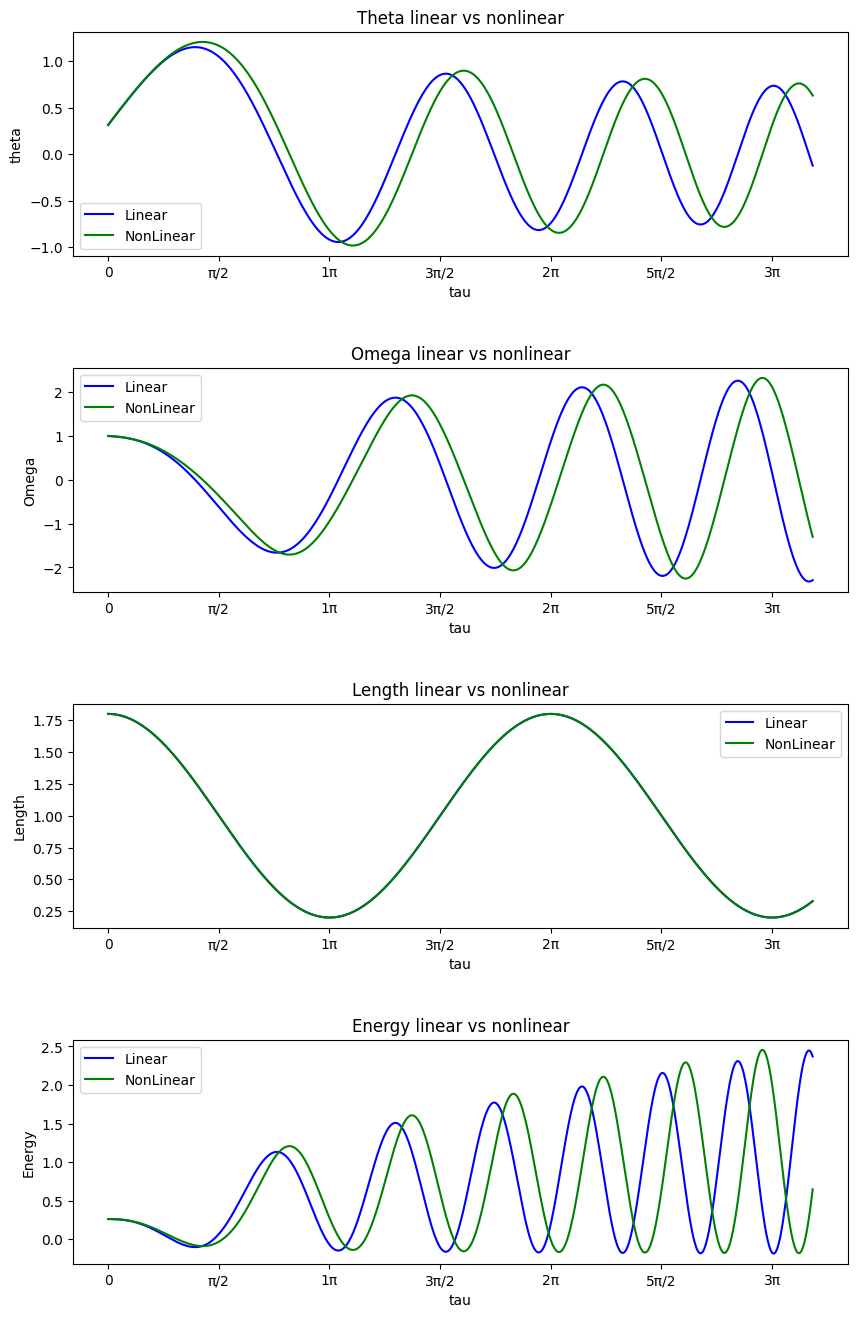
\includegraphics[scale = 0.6]{Images/nonlinear_vs_linear_systems.png}
\caption{Plots to show the difference in the nonlinear versus linear systems. }
\label{png:nonlinear_vs_linear_systems}
\end{figure}

\jump
\begin{figure}[!ht]
\centering
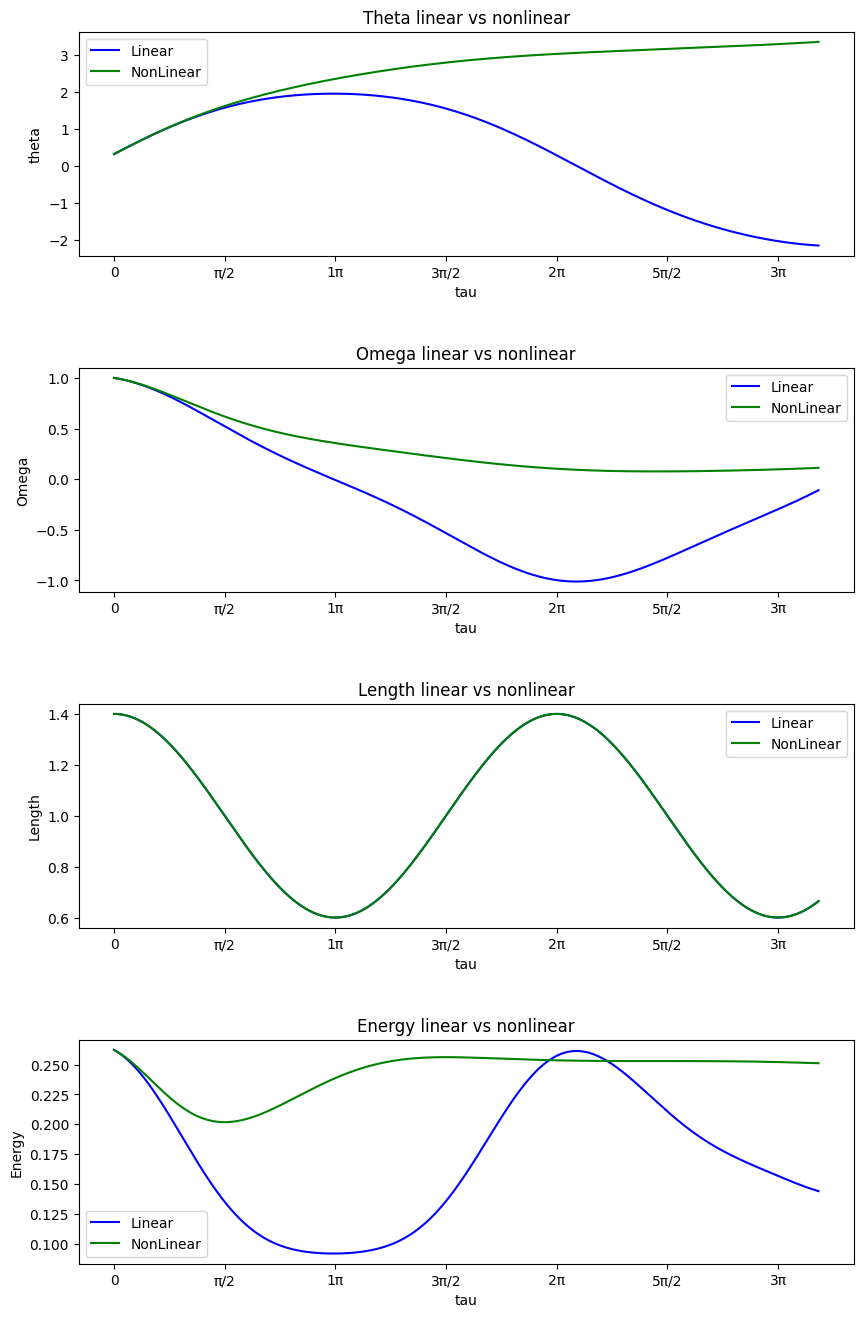
\includegraphics[scale = 0.6]{Images/nonlinear_vs_linear_systems_error.png}
\caption{Error plots, not sure what the problem is. }
\label{png:nonlinear_vs_linear_systems_error}
\end{figure}




\end{enumerate}
<<<<<<< HEAD:Semester 1/Applied Dynamical Systems/Homework1/main.tex
\end{document}
=======
\end{enumerate}
\end{document}
>>>>>>> 6da352df4ff58849a5b0cb34dc1187956b5d693b:main.tex
